%%%%%%%%%%%%%%%%%%%%%%%%%%%%%%%%%%%%%%%%%%%%%%%%%%%%%%%%%%%%%%%%%%%%%%%%%%%%
%%%%%%%%%%%%%%%%%%%%%%%%%%%%%%%%%%%%%%%%%%%%%%%%%%%%%%%%%%%%%%%%%%%%%%%%%%%%
%%%%%%%%%%%%%%%%%%%%%%%%%%%%%%%%%%%%%%%%%%%%%%%%%%%%%%%%%%%%%%%%%%%%%%%%%%%%


%https://texample.net/polarization-controller/
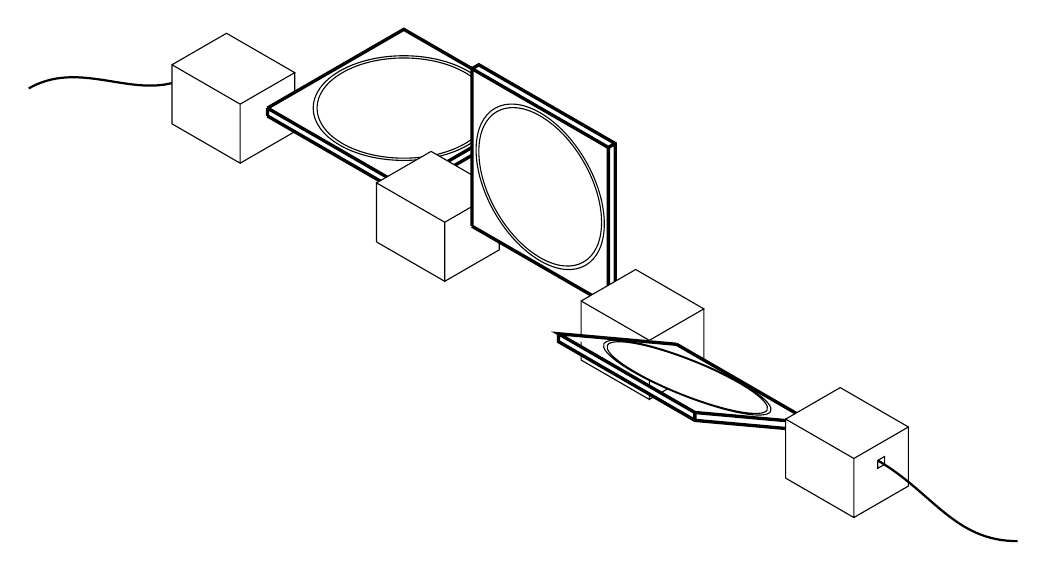
\begin{tikzpicture}[x={(0.866cm,-0.5cm)},
  y={(0.866cm,0.5cm)}, z={(0cm,1cm)}]
\tikzstyle{paddle}=[very thick, fill=white]
\coordinate (O) at (0, 0, 0);

% fiber in
\draw[thick] (0,-1.5,0) to[out=30,in=220] (1,0,0);

% first divider
\draw[fill=white] (1,-.4,-.5) -- (2,-.4,-.5) -- (2,-.4,.25) --
      (1,-.4,.25) -- (1,-.4,-.5)
      (2,-.4,.25) -- (2,.4,.25) -- (1,.4,.25) -- (1,-.4,.25)
      (2,.4,.25) -- (2,.4,-.5) -- (2,-.4,-.5);

% first paddle
\draw[paddle] 
      (2,0,0) -- (4,0,0) -- (4,2,0) -- (2,2,0) -- (2,0,0) % first face
      (2,0,0) -- (2,0,-.1)
      (4,0,0) -- (4,0,-.1)
      (2,0,-.1) -- (4,0,-.1) -- (4,2,-.1);
\draw (3,1,0) circle (.94)
      (3,1,0) circle (.9);

% second divider
\draw[fill=white] (4,-.4,-.5) -- (5,-.4,-.5) -- (5,-.4,.25) -- 
      (4,-.4,.25) -- (4,-.4,-.5)
      (5,-.4,.25) -- (5,.4,.25) -- (4,.4,.25) -- (4,-.4,.25)
      (5,.4,.25) -- (5,.4,-.5) -- (5,-.4,-.5);

% second paddle
\filldraw[paddle]
     (5,0,0) -- (7,0,0) -- (7,0,2) -- (5,0,2) -- (5,0,0) % first face
     (7,0,0) -- (7,.1,0) -- (7,.1,2) -- (5,.1,2) -- (5,0,2)
     (7,.1,2) -- (7,0,2);

% third divider
\draw[fill=white] (7,-.4,-.5) -- (8,-.4,-.5) -- (8,-.4,.25) --
      (7,-.4,.25) -- (7,-.4,-.5)
      (8,-.4,.25) -- (8,.4,.25) -- (7,.4,.25) -- (7,-.4,.25)
      (8,.4,.25) -- (8,.4,-.5) -- (8,-.4,-.5);

% third paddle
\filldraw[paddle] 
     (8,0,0) -- (10,0,0) -- (10, -1.732,1) -- (8,-1.732,1)
     -- (8,0,0)
(8,-1.732,1) -- (8,-1.732,.9) -- (10,-1.732,.9) -- (10,0,-.1)
-- (10,0,0)
(10,-1.732,.9) -- (10,-1.732,1);

% fourth divider  
\draw[fill=white] (10,-.4,-.5) -- (11,-.4,-.5) -- (11,-.4,.25) --
      (10,-.4,.25) -- (10,-.4,-.5)
      (11,-.4,.25) -- (11,.4,.25) -- (10,.4,.25) -- (10,-.4,.25)
      (11,.4,.25) -- (11,.4,-.5) -- (11,-.4,-.5);

\begin{scope}[x={(0.866cm,-0.5cm)},y={(0,1cm)}]
\draw (6,0,1) circle (.94)
      (6,0,1) circle (.9);
\end{scope}

\begin{scope}[x={(0.866cm,-0.5cm)},y={(-.73cm,.077cm)}]
\draw[fill=white] (9,1) circle (.94)
      (9,1) circle (.9);
\end{scope}

% fiber exit
\draw (11,-.05,.05) -- (11,.05,.05) --
     (11,.05,-.05) -- (11,-.05,-.05) -- (11,-.05,.05);
\draw[thick] (10.95,0,0) to[out=-30,in=180] (12,1,-1);
\end{tikzpicture}


%%%%%%%%%%%%%%%%%%%%%%%%%%%%%%%%%%%%%%%%%%%%%%%%%%%%%%%%%%%%%%%%%%%%%%%%%%%%
%%%%%%%%%%%%%%%%%%%%%%%%%%%%%%%%%%%%%%%%%%%%%%%%%%%%%%%%%%%%%%%%%%%%%%%%%%%%
%%%%%%%%%%%%%%%%%%%%%%%%%%%%%%%%%%%%%%%%%%%%%%%%%%%%%%%%%%%%%%%%%%%%%%%%%%%%

%https://texample.net/raindrop/
%\usetikzlibrary{calc,decorations.markings}

% Draw an arc denoting an angle using start and delta angles
\newcommand{\drawarcdelta}[4]{
  \draw ($#1+(#2:#4)$) arc[start angle=#2, delta angle=#3, radius=#4];
}

% Draw an arc with label denoting an angle using start and delta angles
\newcommand{\drawlabeledarcdelta}[6]{
  \drawarcdelta{#1}{#2}{#3}{#4}
  \node at ($#1+(#2+#3/2:#6)$) {#5};
}

\begin{tikzpicture}[xscale=-1,
    ray/.style={decoration={markings,mark=at position .5 with {
      \arrow[>=latex]{>}}},postaction=decorate}
  ]

  % Radius of raindrop
  \pgfmathsetlengthmacro{\r}{3cm}
  % Position where the incoming ray enters the raindrop, as a fraction of
  % the height of the drop.  If 0., the ray will enter in the middle of the
  % drop, if 1., the ray will enter at the top of the drop.
  \pgfmathsetmacro{\f}{.7}

  % Various radii for drawing angle arcs and labels
  \pgfmathsetlengthmacro{\arcradius}{.8cm}
  \pgfmathsetlengthmacro{\dotradius}{.6cm}
  \pgfmathsetlengthmacro{\arclabelradius}{1cm}

  % Calculation of the angle of incidence
  \pgfmathsetmacro{\incidentangle}{asin(\f)}

  % Coordinates of origin and point of entry
  \coordinate (O) at (0, 0);
  \coordinate (A) at (\incidentangle:\r);

  % Draw the drop and the incoming ray, as well as the angle of incidence
  \draw (O) circle (\r);
  \draw[ray] (A  -| \r*3, 0) -- (A);
  \draw[gray] (O) -- ($(O)!1.5!(A)$) node[pos=1.05] {$n$};
  \drawarcdelta{(A)}{0}{\incidentangle}{\arcradius-1pt}
  \drawlabeledarcdelta{(A)}{0}{\incidentangle}{\arcradius+1pt}
    {$i$}{\arclabelradius}

  % For each red and blue ray.  The index of refraction for red light is
  % slightly exaggerated, it should be 1.33.
  \foreach \index/\color in {1.32/red, 1.34/blue} {
    % Calculate angle of refraction
    \pgfmathsetmacro{\refractedangle}{asin(sin(\incidentangle) / \index)}
    % Calculate top angle (at O) in the triangle formed by O, the point of
    % entry, and the point of internal reflection
    \pgfmathsetmacro{\angleindrop}{180 - 2*\refractedangle}

    % Coordinate of point of reflection
    \coordinate (A') at (\incidentangle+\angleindrop:\r);
    % Coordinate of point of exit
    \coordinate (A'') at (\incidentangle+2*\angleindrop:\r);

    \begin{scope}[opacity=.5, color=\color]
      % Draw the light rays
      \draw[ray] (A) -- (A');
      \draw[ray] (A') -- (A'');
      \draw[ray] (A'') -- ($(A'')+(2*\incidentangle+2*\angleindrop:2*\r)$);

      % Draw the normal lines
      \draw (O) -- ($(O)!1.5!(A')$) node[pos=1.05] {$n$};
      \draw (O) -- ($(O)!1.5!(A'')$) node[pos=1.05] {$n$};

      % Draw the arcs and labels
      \drawlabeledarcdelta{(A)}{\incidentangle+180}{-\refractedangle}
        {\arcradius}{$r$}{\arclabelradius}
      \drawarcdelta{(A')}{\incidentangle+\angleindrop+180}{\refractedangle}
        {\arcradius}
      \drawarcdelta{(A')}{\incidentangle+\angleindrop+180}{-\refractedangle}
        {\arcradius}
      \drawarcdelta{(A'')}{\incidentangle+2*\angleindrop+180}{\refractedangle}
        {\arcradius}
    \end{scope}

    % Draw the arcs of the angles of the rays leaving the raindrop.  Note
    % that the angles are identical to the original angle of incidence.
    \drawarcdelta{(A'')}{\incidentangle+2*\angleindrop}{\incidentangle}
      {\arcradius-1pt}
    \drawarcdelta{(A'')}{\incidentangle+2*\angleindrop}{\incidentangle}
      {\arcradius+1pt}
  }

  % Mark the center of the raindrop
  \draw[fill] (O) circle (1.5pt);
\end{tikzpicture}








%%%%%%%%%%%%%%%%%%%%%%%%%%%%%%%%%%%%%%%%%%%%%%%%%%%%%%%%%%%%%%%%%%%%%%%%%%%%
%%%%%%%%%%%%%%%%%%%%%%%%%%%%%%%%%%%%%%%%%%%%%%%%%%%%%%%%%%%%%%%%%%%%%%%%%%%%
%%%%%%%%%%%%%%%%%%%%%%%%%%%%%%%%%%%%%%%%%%%%%%%%%%%%%%%%%%%%%%%%%%%%%%%%%%%%


%https://texample.net/polarizing-microscope/
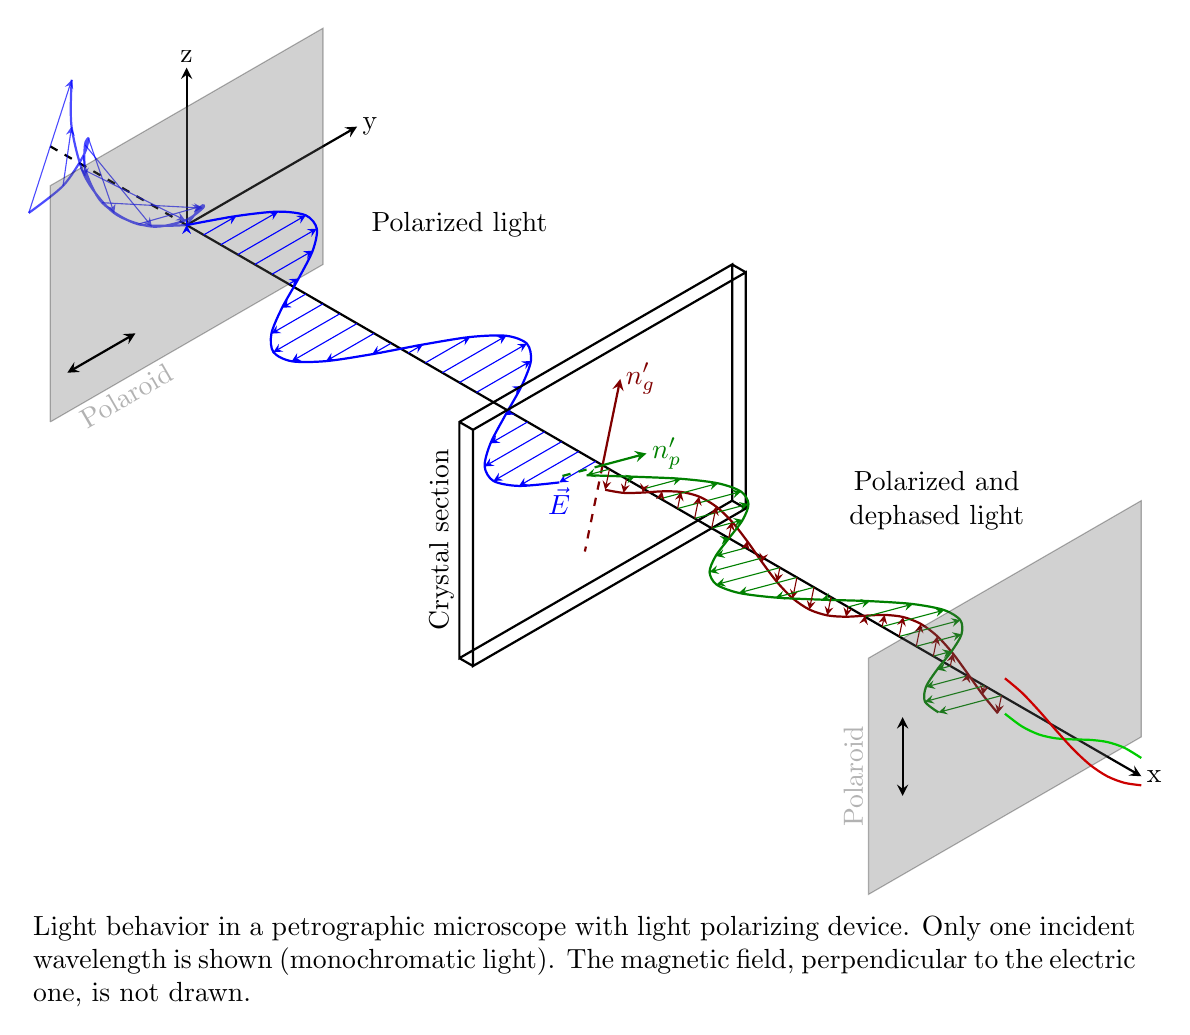
\begin{tikzpicture}[x={(0.866cm,-0.5cm)}, y={(0.866cm,0.5cm)}, z={(0cm,1cm)}, scale=1.0,
    %Option for nice arrows
    >=stealth, %
    inner sep=0pt, outer sep=2pt,%
    axis/.style={thick,->},
    wave/.style={thick,color=#1,smooth},
    polaroid/.style={fill=black!60!white, opacity=0.3},
]
    % Colors
    \colorlet{darkgreen}{green!50!black}
    \colorlet{lightgreen}{green!80!black}
    \colorlet{darkred}{red!50!black}
    \colorlet{lightred}{red!80!black}

    % Frame
    \coordinate (O) at (0, 0, 0);
    \draw[axis] (O) -- +(14, 0,   0) node [right] {x};
    \draw[axis] (O) -- +(0,  2.5, 0) node [right] {y};
    \draw[axis] (O) -- +(0,  0,   2) node [above] {z};

    \draw[thick,dashed] (-2,0,0) -- (O);

    % monochromatic incident light with electric field
    \draw[wave=blue, opacity=0.7, variable=\x, samples at={-2,-1.75,...,0}]
        plot (\x, { cos(1.0*\x r)*sin(2.0*\x r)}, { sin(1.0*\x r)*sin(2.0*\x r)})
        plot (\x, {-cos(1.0*\x r)*sin(2.0*\x r)}, {-sin(1.0*\x r)*sin(2.0*\x r)});

    \foreach \x in{-2,-1.75,...,0}{
        \draw[color=blue, opacity=0.7,->]
            (\x,0,0) -- (\x, { cos(1.0*\x r)*sin(2.0*\x r)}, { sin(1.0*\x r)*sin(2.0*\x r)})
            (\x,0,0) -- (\x, {-cos(1.0*\x r)*sin(2.0*\x r)}, {-sin(1.0*\x r)*sin(2.0*\x r)});
    }

    \filldraw[polaroid] (0,-2,-1.5) -- (0,-2,1.5) -- (0,2,1.5) -- (0,2,-1.5) -- (0,-2,-1.5)
        node[below, sloped, near end]{Polaroid};%

    %Direction of polarization
    \draw[thick,<->] (0,-1.75,-1) -- (0,-0.75,-1);

    % Electric field vectors
    \draw[wave=blue, variable=\x,samples at={0,0.25,...,6}]
        plot (\x,{sin(2*\x r)},0)node[anchor=north]{$\vec{E}$};

    %Polarized light between polaroid and thin section
    \foreach \x in{0, 0.25,...,6}
        \draw[color=blue,->] (\x,0,0) -- (\x,{sin(2*\x r)},0);

    \draw (3,1,1) node [text width=2.5cm, text centered]{Polarized light};

    %Crystal thin section
    \begin{scope}[thick]
        \draw (6,-2,-1.5) -- (6,-2,1.5) node [above, sloped, midway]{Crystal section}
                -- (6, 2, 1.5) -- (6, 2, -1.5) -- cycle % First face
            (6,  -2, -1.5) -- (6.2, -2,-1.5)
            (6,   2, -1.5) -- (6.2,  2,-1.5)
            (6,  -2,  1.5) -- (6.2, -2, 1.5)
            (6,   2,  1.5) -- (6.2,  2, 1.5)
            (6.2,-2, -1.5) -- (6.2, -2, 1.5) -- (6.2, 2, 1.5) 
                -- (6.2, 2, -1.5) -- cycle; % Second face

        %Optical indices
        \draw[darkred, ->]       (6.1, 0, 0) -- (6.1, 0.26,  0.966) node [right] {$n_{g}'$}; % index 1
        \draw[darkred, dashed]   (6.1, 0, 0) -- (6.1,-0.26, -0.966); % index 1
        \draw[darkgreen, ->]     (6.1, 0, 0) -- (6.1, 0.644,-0.173) node [right] {$n_{p}'$}; % index 2
        \draw[darkgreen, dashed] (6.1, 0, 0) -- (6.1,-0.644, 0.173); % index 2
    \end{scope}

    %Rays leaving thin section
    \draw[wave=darkred,   variable=\x, samples at={6.2,6.45,...,12}] 
        plot (\x, {0.26*0.26*sin(2*(\x-0.5) r)},  {0.966*0.26*sin(2*(\x-0.5) r)});  %n'g-oriented ray
    \draw[wave=darkgreen, variable=\x, samples at={6.2,6.45,...,12}]
        plot (\x, {0.966*0.966*sin(2*(\x-0.1) r)},{-0.26*0.966*sin(2*(\x-0.1) r)}); %n'p-oriented ray
    \draw (10,1,1) node [text width=2.5cm, text centered] {Polarized and dephased light};

    \foreach \x in{6.2,6.45,...,12} {
        \draw[color=darkgreen, ->] (\x, 0, 0) --
            (\x, {0.966*0.966*sin(2*(\x-0.1) r)}, {-0.26*0.966*sin(2*(\x-0.1) r)});
        \draw[color=darkred,   ->] (\x, 0, 0) --
            (\x, {0.26*0.26*sin(2*(\x-0.5) r)}, {0.966*0.26*sin(2*(\x-0.5) r)});
    }

    %Second polarization
    \draw[polaroid]   (12, -2,  -1.5) -- (12, -2,   1.5)  %Polarizing filter
        node [above, sloped,midway] {Polaroid} -- (12, 2, 1.5) -- (12, 2, -1.5) -- cycle;
    \draw[thick, <->] (12, -1.5,-0.5) -- (12, -1.5, 0.5); %Polarization direction

    %Light leaving the second polaroid
    \draw[wave=lightgreen,variable=\x, samples at={12, 12.25,..., 14}]
        plot (\x,{0}, {0.966*0.966*0.26*sin(2*(\x-0.5) r)}); %n'g polarized ray
    \draw[wave=lightred,  variable=\x, samples at={12, 12.25,..., 14}]
        plot (\x,{0}, {-0.26*0.966*sin(2*(\x-0.1) r)});      %n'p polarized ray

    \node[align=justify, text width=14cm, anchor=north west, yshift=-2mm] at (current bounding box.south west)
        {Light behavior in a petrographic microscope with light polarizing
        device. Only one incident wavelength is shown (monochromatic light).
        The magnetic field, perpendicular to the electric one, is not drawn.};
\end{tikzpicture}






%%%%%%%%%%%%%%%%%%%%%%%%%%%%%%%%%%%%%%%%%%%%%%%%%%%%%%%%%%%%%%%%%%%%%%%%%%%%
%%%%%%%%%%%%%%%%%%%%%%%%%%%%%%%%%%%%%%%%%%%%%%%%%%%%%%%%%%%%%%%%%%%%%%%%%%%%
%%%%%%%%%%%%%%%%%%%%%%%%%%%%%%%%%%%%%%%%%%%%%%%%%%%%%%%%%%%%%%%%%%%%%%%%%%%%

%https://tikz.net/electromagnetic_wave/
\colorlet{myblue}{black!40!blue}
\colorlet{myred}{black!40!red}
\colorlet{vcol}{green!50!black}
\colorlet{Ecol}{orange!90!black}
\colorlet{EVcol}{orange!80!black!60}
\colorlet{Bcol}{violet!90}
% Electromagnetic wave - colored
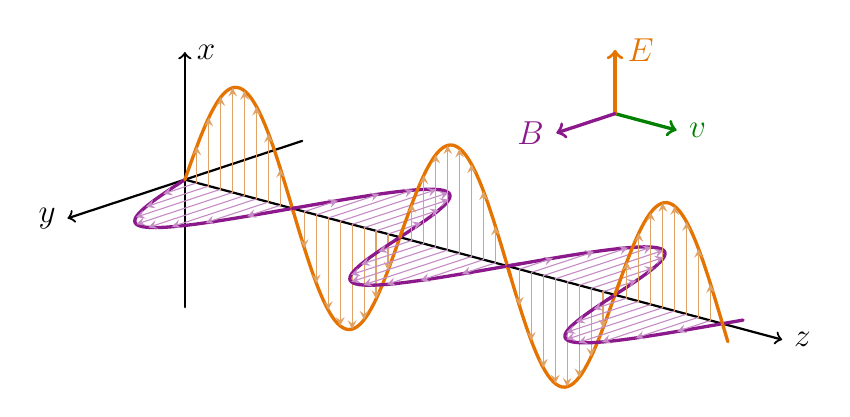
\begin{tikzpicture}[x=(-15:0.9), y=(90:0.9), z=(-150:1.1),
                    line cap=round, line join=round,
                    axis/.style={black, thick,->},
                    vector/.style={>=stealth,->}]
  \large
  \def\A{1.5}
  \def\nNodes{5} % use even number
  \def\nVectorsPerNode{8}
  \def\N{\nNodes*40}
  \def\xmax{\nNodes*pi/2*1.01}
  \pgfmathsetmacro\nVectors{(\nVectorsPerNode+1)*\nNodes}
  \def\vE{{\color{Ecol}\mathbf{E}}}
  \def\vB{{\color{Bcol}\mathbf{B}}}
  
  \def\drawENode{ % draw E node and vectors with some offset
    \draw[Ecol,very thick,variable=\t,domain=\iOffset*pi/2:(\iOffset+1)*pi/2*1.01,samples=40]
      plot (\t,{\A*sin(\t*360/pi)},0);
    \foreach \k [evaluate={\t=\k*pi/2/(\nVectorsPerNode+1);
                           \angle=\k*90/(\nVectorsPerNode+1);}]
                in {1,...,\nVectorsPerNode}{
      \draw[vector,EVcol]  (\iOffset*pi/2+\t,0,0) -- ++(0,{\A*sin(2*\angle+\iOffset*180)},0);
    }
  }
  \def\drawBNode{ % draw B node and vectors with some offset
    \draw[Bcol,very thick,variable=\t,domain=\iOffset*pi/2:(\iOffset+1)*pi/2*1.01,samples=40]
      plot (\t,0,{\A*sin(\t*360/pi)});
    \foreach \k [evaluate={\t=\k*pi/2/(\nVectorsPerNode+1);
                           \angle=\k*90/(\nVectorsPerNode+1);}]
                in {1,...,\nVectorsPerNode}{
      \draw[vector,Bcol!50]  (\iOffset*pi/2+\t,0,0) -- ++(0,0,{\A*sin(2*\angle+\iOffset*180)});
    }
  }
  
  % MAIN AXES
  \draw[axis] (0,0,0) -- ++(\xmax*1.1,0,0) node[right] {$z$};
  \draw[axis] (0,-\A*1.2,0) -- (0,\A*1.2,0) node[right] {$x$};
  \draw[axis] (0,0,-\A*1.2) -- (0,0,\A*1.2) node[left] {$y$};
  
  % SMALL AXES
  \def\xOffset{{(\nNodes-2)*pi/2}}
  \def\yOffset{\A*1.1}
  \def\zOffset{\A*1.1}
  \draw[axis,very thick,vcol] (\xOffset,\yOffset,-\zOffset) -- ++(\A*0.6,0,0) node[right,align=center] {$\vb{v}$}; %\\propagation
  \draw[axis,very thick,Ecol]  (\xOffset,\yOffset,-\zOffset) -- ++(0,\A*0.6,0) node[right] {$\vb{E}$};
  \draw[axis,very thick,Bcol]   (\xOffset,\yOffset,-\zOffset) -- ++(0,0,\A*0.6) node[left] {$\vb{B}$};
  
  % draw (anti-)nodes
  \foreach \iNode [evaluate={\iOffset=\iNode-1;}] in {1,...,\nNodes}{
    \ifodd\iNode \drawBNode \drawENode % E overlaps B
    \else        \drawENode \drawBNode % B overlaps E
    \fi
  }

\end{tikzpicture}



% Electromagnetic wave - circular polarization - color
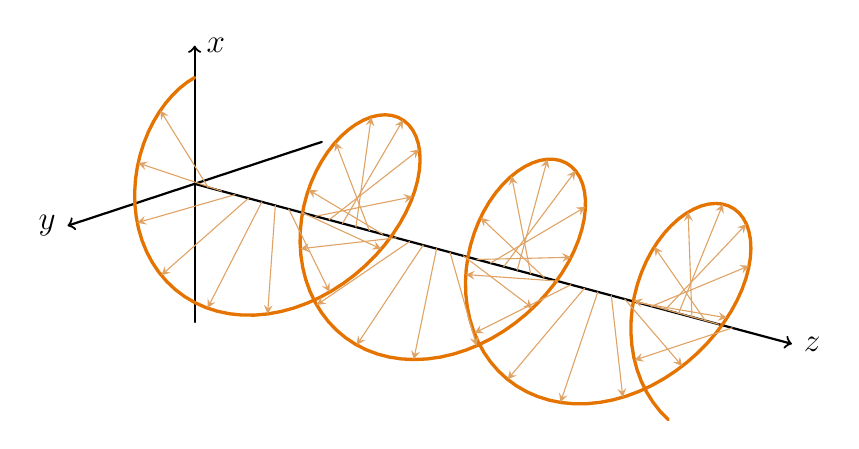
\begin{tikzpicture}[x=(-15:0.9), y=(90:0.9), z=(-150:1.1),
                    line cap=round, line join=round,
                    axis/.style={black, thick,->},
                    vector/.style={>=stealth,->}]
  
  \large
  \def\A{1.5}
  \def\om{1.3}
  \def\nNodes{5} % use even number
  \def\nVectorsPerNode{8}
  \def\N{\nNodes*40}
  \def\xmax{\nNodes*pi/2*1.01}
  \pgfmathsetmacro\nVectors{\nVectorsPerNode*\nNodes}
  \def\vE{\mathbf{E}}
  \def\vB{\mathbf{B}}
  
  % MAIN AXES
  \draw[axis] (0,0,0) -- ++(\xmax*1.1,0,0) node[right] {$z$};
  \draw[axis] (0,-\A*1.3,0) -- (0,\A*1.3,0) node[right] {$x$};
  \draw[axis] (0,0,-\A*1.3) -- (0,0,\A*1.3) node[left] {$y$};
  
  % waves
  \draw[Ecol,very thick,variable=\t,domain=0:\nNodes*pi/2*1.03,samples=\N]
    plot (\t,{\A*cos(\om*\t*360/pi)},{\A*sin(\om*\t*360/pi)});
  
  % draw vectors
  \foreach \k [evaluate={\t=\k*pi/2/\nVectorsPerNode;
                         \angle=\k*90/\nVectorsPerNode;}]
              in {1,...,\nVectors}{
    \draw[EVcol,vector] (\t,0,0) -- ++(0,{\A*cos(\om*2*\angle)},{\A*sin(\om*2*\angle)});
  }
  
\end{tikzpicture}



% Electromagnetic wave SHORT - colored
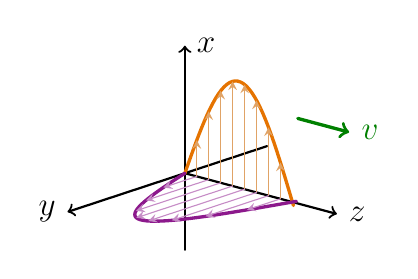
\begin{tikzpicture}[x=(-15:0.9), y=(90:0.9), z=(-150:1.1),
                    line cap=round, line join=round,
                    axis/.style={black, thick,->},
                    vector/.style={>=stealth,->}]
  \large
  \def\A{1.5}
  \def\ymax{1.8}
  \def\nNodes{1} % use even number
  \def\nVectorsPerNode{8}
  \def\N{\nNodes*40}
  \def\xmax{\nNodes*pi/2*1.01}
  \pgfmathsetmacro\nVectors{(\nVectorsPerNode+1)*\nNodes}
  
  % MAIN AXES
  \draw[axis] (0,0,0) -- ++(\xmax*1.4,0,0) node[right] {$z$};
  \draw[axis] (0,-\ymax*0.6,0) -- (0,\ymax,0) node[right] {$x$};
  \draw[axis] (0,0,-\ymax*0.7) -- (0,0,\ymax) node[left] {$y$};
  
  \draw[Ecol,very thick,variable=\t,domain=0:pi/2*1.01,samples=40]
    plot (\t,{\A*sin(\t*360/pi)},0);
  \foreach \k [evaluate={\t=\k*pi/2/(\nVectorsPerNode+1);
                         \angle=\k*90/(\nVectorsPerNode+1);}]
              in {1,...,\nVectorsPerNode}{
    \draw[vector,EVcol]  (\t,0,0) -- ++(0,{\A*sin(2*\angle)},0);
  }
  \draw[Bcol,very thick,variable=\t,domain=0:pi/2*1.01,samples=40]
    plot (\t,0,{\A*sin(\t*360/pi)});
  \foreach \k [evaluate={\t=\k*pi/2/(\nVectorsPerNode+1);
                         \angle=\k*90/(\nVectorsPerNode+1);}]
              in {1,...,\nVectorsPerNode}{
    \draw[vector,Bcol!50]  (\t,0,0) -- ++(0,0,{\A*sin(2*\angle)});
  }
  
  % VECTOR
  \draw[->,very thick,vcol] (\A*1.1,\A*0.8,0) --++ (\A*0.5,0,0) node[right] {$\vb{v}$};
  
\end{tikzpicture}



% Electromagnetic wave SHORT SQUARED - colored
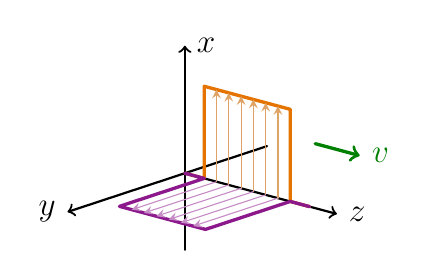
\begin{tikzpicture}[x=(-15:0.9), y=(90:0.9), z=(-150:1.1),
                    line cap=round, line join=round,
                    axis/.style={black, thick,->},
                    vector/.style={>=stealth,->}]
  \large
  \def\A{1.3}
  \def\ymax{1.8}
  \def\nNodes{1} % use even number
  \def\nVectorsPerNode{6}
  \def\N{\nNodes*40}
  \def\xmax{\nNodes*pi/2*1.01}
  \def\wx{\nNodes*pi/2*0.8}
  \def\dx{\nNodes*pi/2*0.18}
  \pgfmathsetmacro\nVectors{(\nVectorsPerNode+1)*\nNodes}
  
  % MAIN AXES
  \draw[axis] (0,0,0) -- ++(\xmax*1.4,0,0) node[right] {$z$};
  \draw[axis] (0,-\ymax*0.6,0) -- (0,\ymax,0) node[right] {$x$};
  \draw[axis] (0,0,-\ymax*0.7) -- (0,0,\ymax) node[left] {$y$};
  
  % IMPULSE
  \draw[Ecol,very thick]
    (0,0,0) --++ (\dx,0,0) --++ (0,\A,0) --++ (\wx,0,0) --++ (0,-\A,0) --++ (\dx,0,0);
  \foreach \k [evaluate={\t=\dx+\k*\wx/(\nVectorsPerNode+1);}] in {1,...,\nVectorsPerNode}{
    \draw[vector,EVcol] (\t,0,0) -- ++(0,\A,0);
  }
  \draw[Bcol,very thick]
    (0,0,0) --++ (\dx,0,0) --++ (0,0,\A) --++ (\wx,0,0) --++ (0,0,-\A) --++ (\dx,0,0);
  \foreach \k [evaluate={\t=\dx+\k*\wx/(\nVectorsPerNode+1);}] in {1,...,\nVectorsPerNode}{
    \draw[vector,Bcol!50] (\t,0,0) -- ++(0,0,\A);
  }
  
  % VECTOR
  \draw[->,very thick,vcol] (\xmax*1.2,\A*0.7,0) --++ (\A*0.5,0,0) node[right] {$\vb{v}$};
  
\end{tikzpicture}



% Electromagnetic wave - black
\begin{tikzpicture}[x=(-15:1.2), y=(90:1.0), z=(-150:1.0),
                    line cap=round, line join=round,
                    axis/.style={black, thick,->},
                    vector/.style={>=stealth,->}]
  \large
  \def\A{1.5}
  \def\nNodes{5} % use even number
  \def\nVectorsPerNode{8}
  \def\N{\nNodes*40}
  \def\xmax{\nNodes*pi/2*1.01}
  \pgfmathsetmacro\nVectors{(\nVectorsPerNode+1)*\nNodes}
  
  \def\vE{\mathbf{E}}
  \def\vB{\mathbf{B}}
  \def\vk{\mathbf{\hat{k}}}
  
  % MAIN AXES
  \draw[axis] (0,0,0) -- ++(\xmax*1.1,0,0) node[right] {$x$};
  \draw[axis] (0,-\A*1.4,0) -- (0,\A*1.4,0) node[right] {$y$};
  \draw[axis] (0,0,-\A*1.4) -- (0,0,\A*1.4) node[above left] {$z$};
  
  % SMALL AXES
  \def\xOffset{{(\nNodes-2)*pi/2}}
  \def\yOffset{\A*1.2}
  \def\zOffset{\A*1.2}
  \draw[axis] (\xOffset,\yOffset,-\zOffset) -- ++(\A*0.6,0,0) node[right] {$\vk$};
  \draw[axis] (\xOffset,\yOffset,-\zOffset) -- ++(0,\A*0.6,0) node[right] {$\vE$};
  \draw[axis] (\xOffset,\yOffset,-\zOffset) -- ++(0,0,\A*0.6) node[above left] {$\vB$};
  
  % equation
  \node[above right] at (\xOffset,-0.5*\yOffset,4*\zOffset)
    {$\begin{aligned}
      \vE &= \mathbf{E_0}\sin(\vk\cdot\mathbf{x}-c_0t)\\
      \vB &= \mathbf{B_0}\sin(\vk\cdot\mathbf{x}-c_0t)\\
      \end{aligned}$};
  \node[below right] at (\xOffset,-0.5*\yOffset,4*\zOffset)
    {$\vE\cdot\vk = 0,\;\; \vB\cdot\vk = 0,\;\; \vB = \frac{1}{c_0}\vk\times\vE$};
  
  % waves
  \draw[very thick,variable=\t,domain=0:\nNodes*pi/2*1.01,samples=\N]
    plot (\t,{\A*sin(\t*360/pi)},0);
  \draw[very thick,variable=\t,domain=0:\nNodes*pi/2*1.01,samples=\N]
    plot (\t,0,{\A*sin(\t*360/pi)});
  
  % draw vectors
  \foreach \k [evaluate={\t=\k*pi/2/(\nVectorsPerNode+1);
                         \angle=\k*90/(\nVectorsPerNode+1);
                         \c=(mod(\angle,90)!=0);}]
              in {1,...,\nVectors}{
    \if\c1
      \draw[vector] (\t,0,0) -- ++(0,{\A*sin(2*\angle)},0);
      \draw[vector] (\t,0,0) -- ++(0,0,{\A*sin(2*\angle)});
    \fi
  }
  
\end{tikzpicture}



% Electromagnetic wave - circular polarization
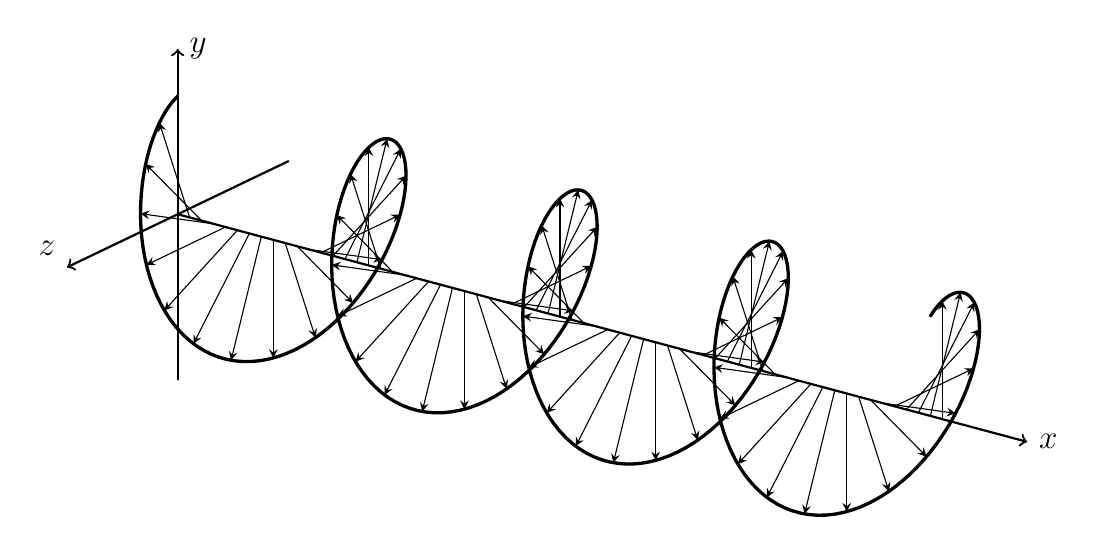
\begin{tikzpicture}[x=(-15:0.8), y=(90:1.0), z=(-150:1.0),
                    line cap=round, line join=round,
                    axis/.style={black, thick,->},
                    vector/.style={>=stealth,->}]
  \large
  \def\A{1.5}
  \def\nNodes{8} % use even number
  \def\nVectorsPerNode{8}
  \def\N{\nNodes*40}
  \def\xmax{\nNodes*pi/2*1.01}
  \pgfmathsetmacro\nVectors{\nVectorsPerNode*\nNodes}
  
  \def\vE{\mathbf{E}}
  \def\vB{\mathbf{B}}
  \def\vk{\mathbf{\hat{k}}}
  
  % MAIN AXES
  \draw[axis] (0,0,0) -- ++(\xmax*1.1,0,0) node[right] {$x$};
  \draw[axis] (0,-\A*1.4,0) -- (0,\A*1.4,0) node[right] {$y$};
  \draw[axis] (0,0,-\A*1.4) -- (0,0,\A*1.4) node[above left] {$z$};
  
  % waves
  \draw[very thick,variable=\t,domain=0:\nNodes*pi/2*1.01,samples=\N]
    plot (\t,{\A*cos(\t*360/pi)},{\A*sin(\t*360/pi)});
  
  % draw vectors
  \foreach \k [evaluate={\t=\k*pi/2/\nVectorsPerNode;
                         \angle=\k*90/\nVectorsPerNode;}]
              in {1,...,\nVectors}{
    \draw[vector] (\t,0,0) -- ++(0,{\A*cos(2*\angle)},{\A*sin(2*\angle)});
  }
  
\end{tikzpicture}



% Electromagnetic wave - colored
\begin{tikzpicture}[x=(-15:1.2), y=(90:1.0), z=(-150:1.0),
                    line cap=round, line join=round,
                    axis/.style={black, thick,->},
                    vector/.style={>=stealth,->}]
  \large
  \def\A{1.5}
  \def\nNodes{5} % use even number
  \def\nVectorsPerNode{8}
  \def\N{\nNodes*40}
  \def\xmax{\nNodes*pi/2*1.01}
  \pgfmathsetmacro\nVectors{(\nVectorsPerNode+1)*\nNodes}
  
  \def\vE{{\color{myblue}\mathbf{E}}}
  \def\vB{{\color{myred}\mathbf{B}}}
  \def\vk{\mathbf{\hat{k}}}
  
  \def\drawENode{ % draw E node and vectors with some offset
    \draw[myblue,very thick,variable=\t,domain=\iOffset*pi/2:(\iOffset+1)*pi/2*1.01,samples=40]
      plot (\t,{\A*sin(\t*360/pi)},0);
    \foreach \k [evaluate={\t=\k*pi/2/(\nVectorsPerNode+1);
                           \angle=\k*90/(\nVectorsPerNode+1);}]
                in {1,...,\nVectorsPerNode}{
      \draw[vector,myblue!50]  (\iOffset*pi/2+\t,0,0) -- ++(0,{\A*sin(2*\angle+\iOffset*180)},0);
    }
  }
  \def\drawBNode{ % draw B node and vectors with some offset
    \draw[myred,very thick,variable=\t,domain=\iOffset*pi/2:(\iOffset+1)*pi/2*1.01,samples=40]
      plot (\t,0,{\A*sin(\t*360/pi)});
    \foreach \k [evaluate={\t=\k*pi/2/(\nVectorsPerNode+1);
                           \angle=\k*90/(\nVectorsPerNode+1);}]
                in {1,...,\nVectorsPerNode}{
      \draw[vector,myred!50]  (\iOffset*pi/2+\t,0,0) -- ++(0,0,{\A*sin(2*\angle+\iOffset*180)});
    }
  }
  
  % MAIN AXES
  \draw[axis] (0,0,0) -- ++(\xmax*1.1,0,0) node[right] {$x$};
  \draw[axis] (0,-\A*1.4,0) -- (0,\A*1.4,0) node[right] {$y$};
  \draw[axis] (0,0,-\A*1.4) -- (0,0,\A*1.4) node[above left] {$z$};
  
  % SMALL AXES
  \def\xOffset{{(\nNodes-2)*pi/2}}
  \def\yOffset{\A*1.2}
  \def\zOffset{\A*1.2}
  \draw[axis,black] (\xOffset,\yOffset,-\zOffset) -- ++(\A*0.6,0,0) node[right,align=center] {$\mathbf{\hat{k}}$}; %\\propagation
  \draw[axis,myblue]  (\xOffset,\yOffset,-\zOffset) -- ++(0,\A*0.6,0) node[right] {$\mathbf{E}$};
  \draw[axis,myred]   (\xOffset,\yOffset,-\zOffset) -- ++(0,0,\A*0.6) node[above left] {$\mathbf{B}$};
  
  % equation
  \node[above right] at (\xOffset,-0.5*\yOffset,4*\zOffset)
    {$\begin{aligned}
      \vE &= {\color{myblue}\mathbf{E_0}}\sin(\vk\cdot\mathbf{x}-c_0t)\\
      \vB &= {\color{myred} \mathbf{B_0}}\sin(\vk\cdot\mathbf{x}-c_0t)\\
      \end{aligned}$};
  \node[below right] at (\xOffset,-0.5*\yOffset,4*\zOffset)
    {$\vE\cdot\vk = 0,\;\; \vB\cdot\vk = 0,\;\; \vB = \frac{1}{c_0}\vk\times\vE$};
  
  % draw (anti-)nodes
  \foreach \iNode [evaluate={\iOffset=\iNode-1;}] in {1,...,\nNodes}{
    \ifodd\iNode \drawBNode \drawENode % E overlaps B
    \else        \drawENode \drawBNode % B overlaps E
    \fi
  }

\end{tikzpicture}

%%%%%%%%%%%%%%%%%%%%%%%%%%%%%%%%%%%%%%%%%%%%%%%%%%%%%%%%%%%%%%%%%%%%%%%%%%%%
%%%%%%%%%%%%%%%%%%%%%%%%%%%%%%%%%%%%%%%%%%%%%%%%%%%%%%%%%%%%%%%%%%%%%%%%%%%%
%%%%%%%%%%%%%%%%%%%%%%%%%%%%%%%%%%%%%%%%%%%%%%%%%%%%%%%%%%%%%%%%%%%%%%%%%%%%

